\documentclass{article}

% Packages for setting up page margins
\usepackage[margin=1in]{geometry}

\usepackage{graphicx, setspace, amsmath, mathtools, amssymb, url, float}
\setlength{\parskip}{2mm}
\graphicspath{ {./images/} }

% Title
\title{CS451 Introduction to Parallel and Distributed Computing - Assignment 5}
\author{Batkhishig Dulamsurankhor - A20543498}
\date{\today} % Use \date{} for no date

\begin{document}

\maketitle

Part 1

14) a. i. yarn node -list

\begin{figure}[H]
  \centering
  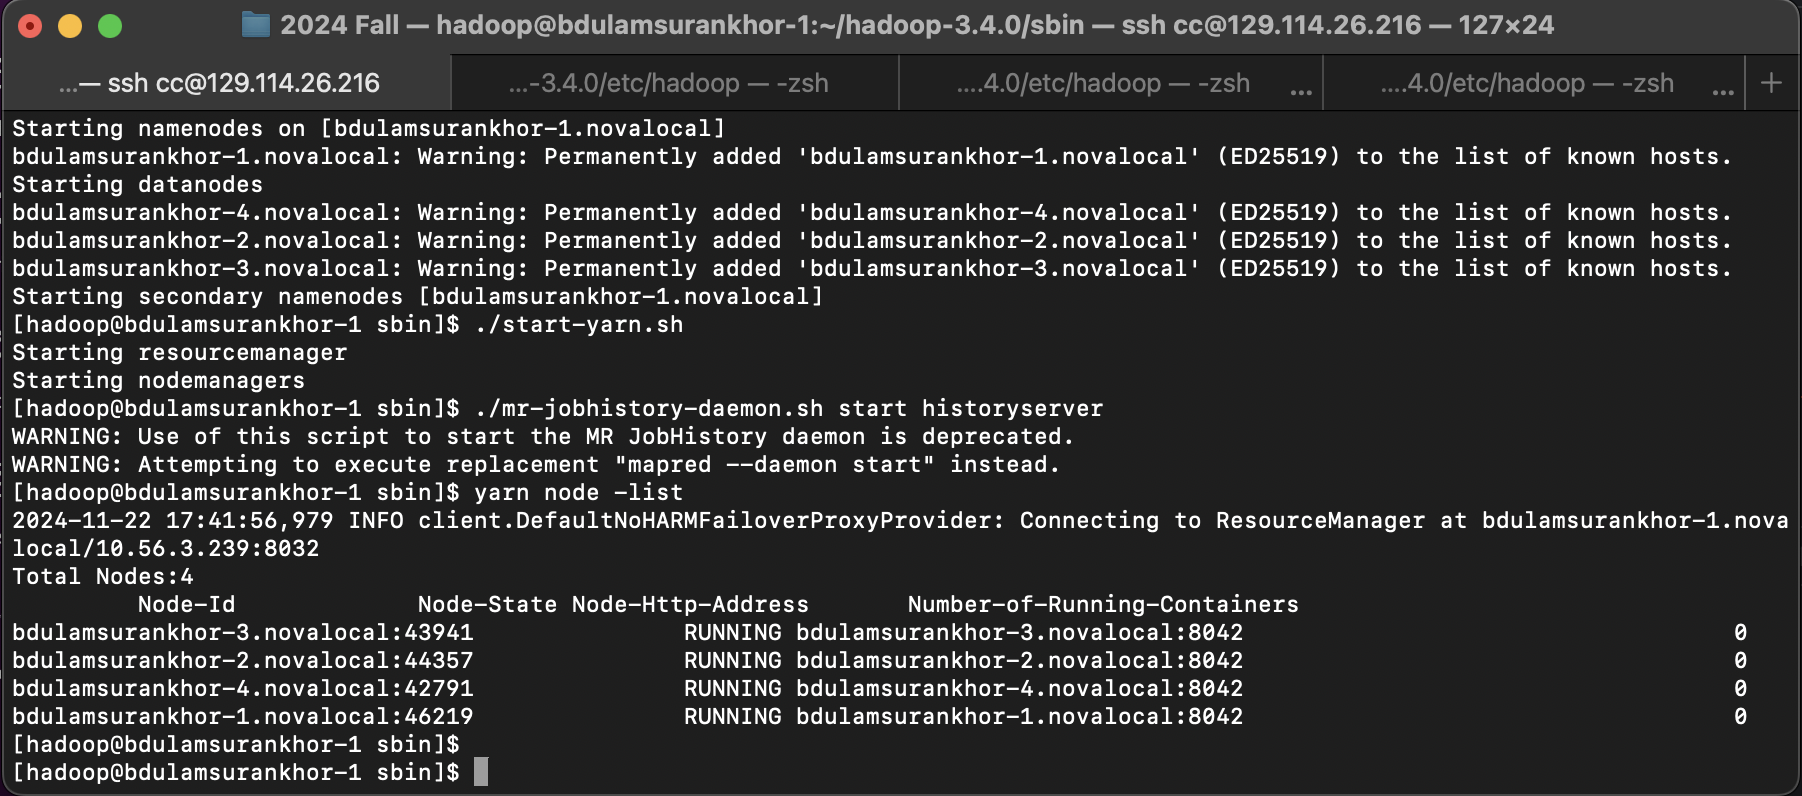
\includegraphics[width=\textwidth]{image1.png}
\end{figure}

Part 2

4) Verify that the file was uploaded to HDFS by hadoop fs -ls /data
\begin{figure}[H]
  \centering
  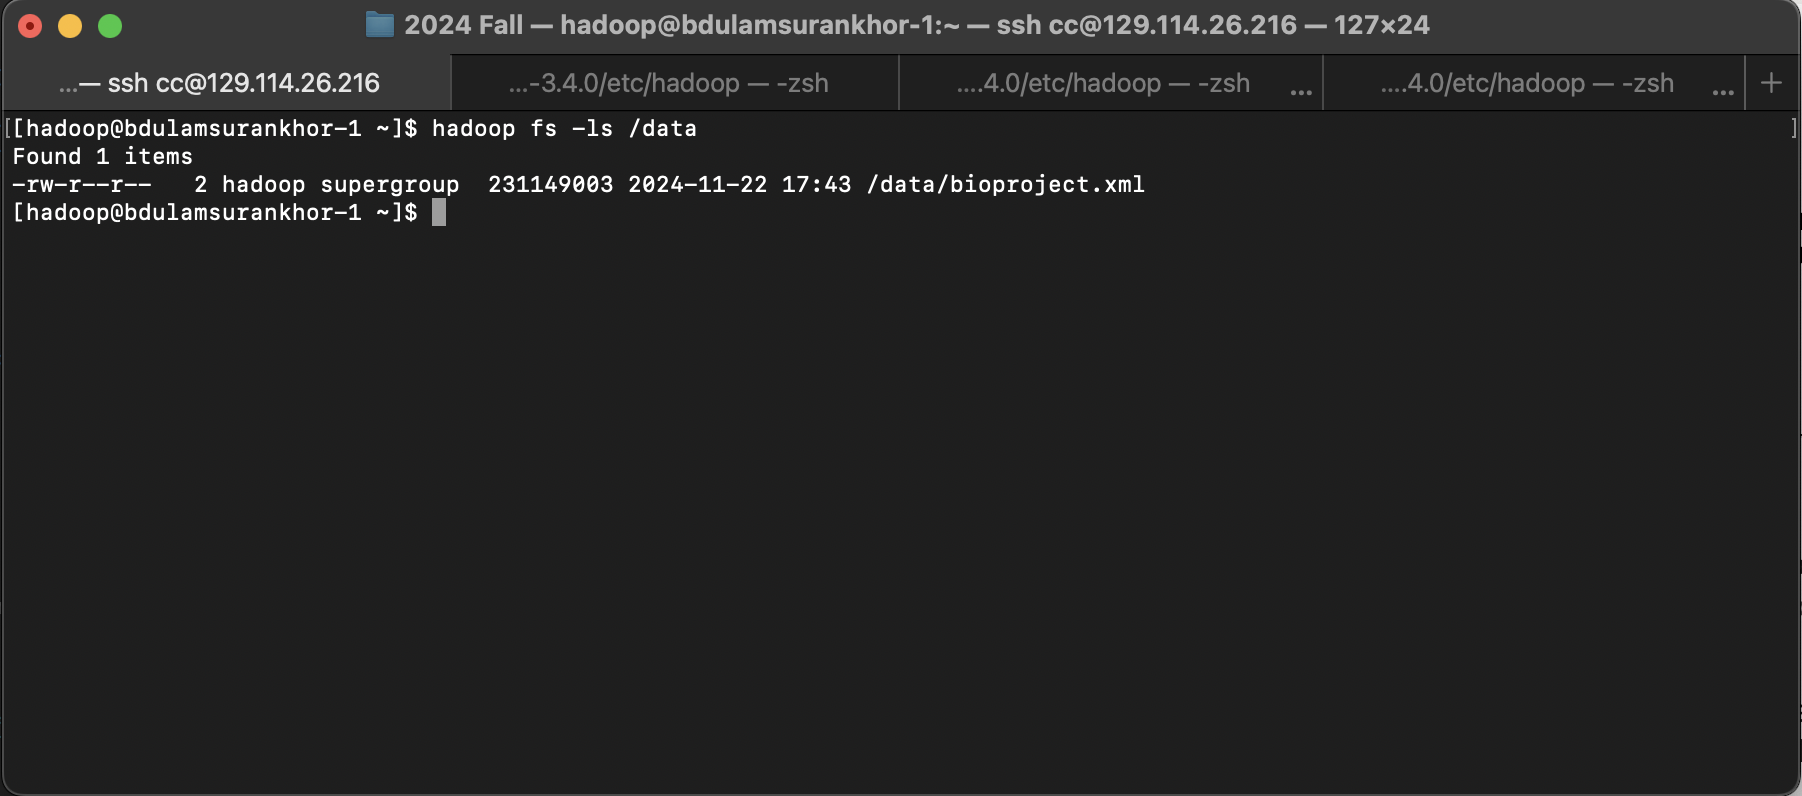
\includegraphics[width=\textwidth]{image2.png}
\end{figure}

5) time hadoop jar hadoop-3.4.0/share/hadoop/mapreduce/hadoop-mapreduce-examples-3.4.0.jar wordcount /data/bioproject.xml /data/wordcount1

\begin{figure}[H]
  \centering
  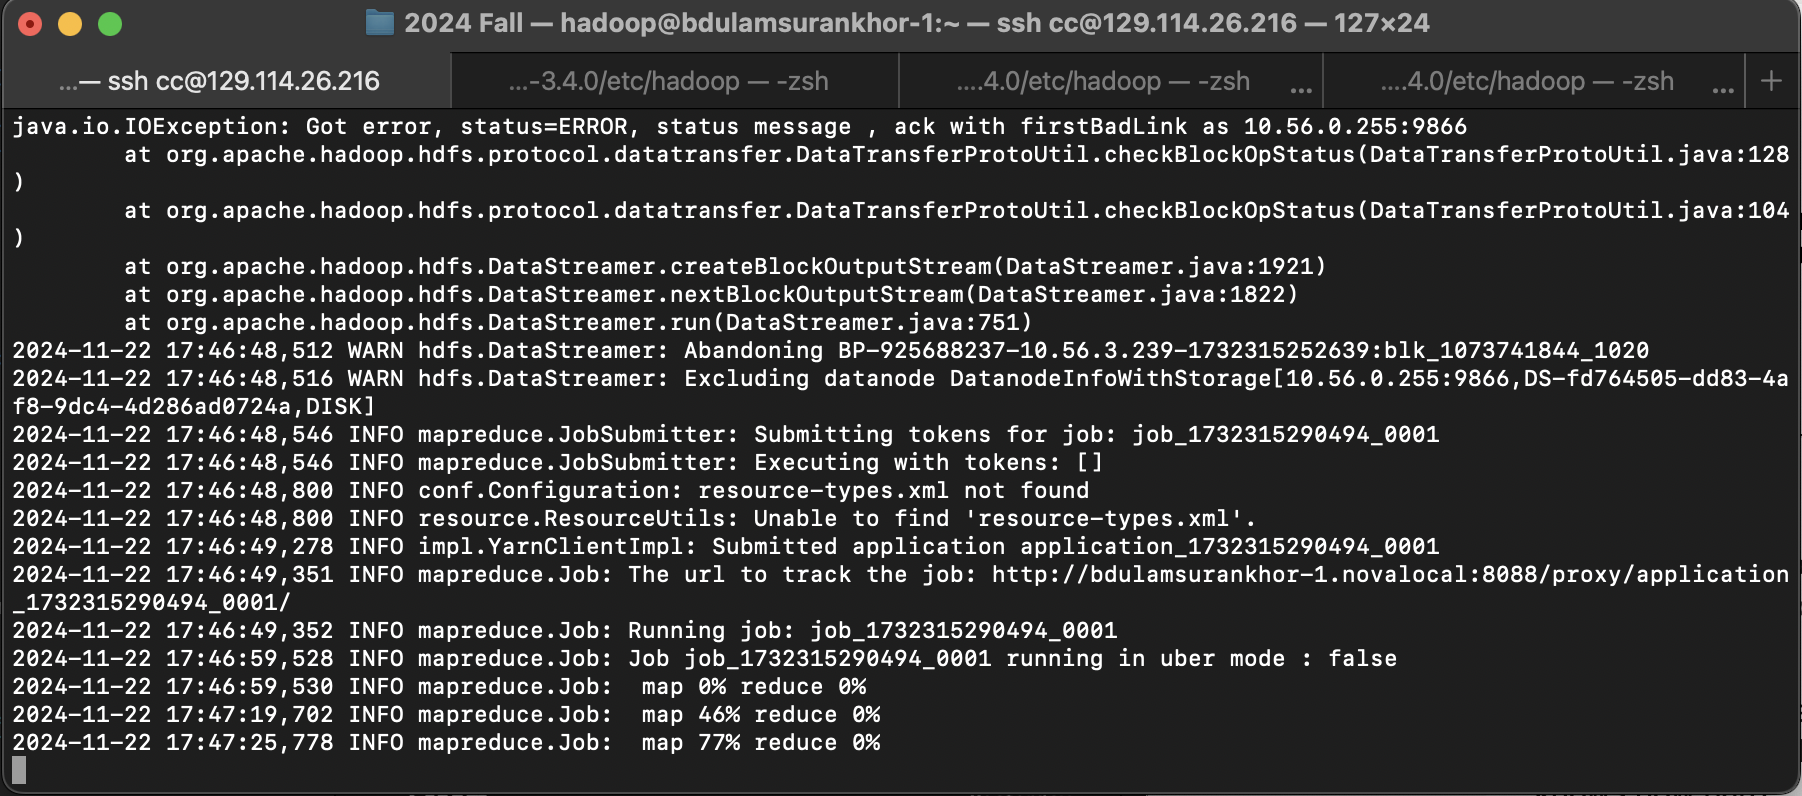
\includegraphics[width=\textwidth]{image3.png}
\end{figure}

hadoop fs -du /data/wordcount1/

\begin{figure}[H]
  \centering
  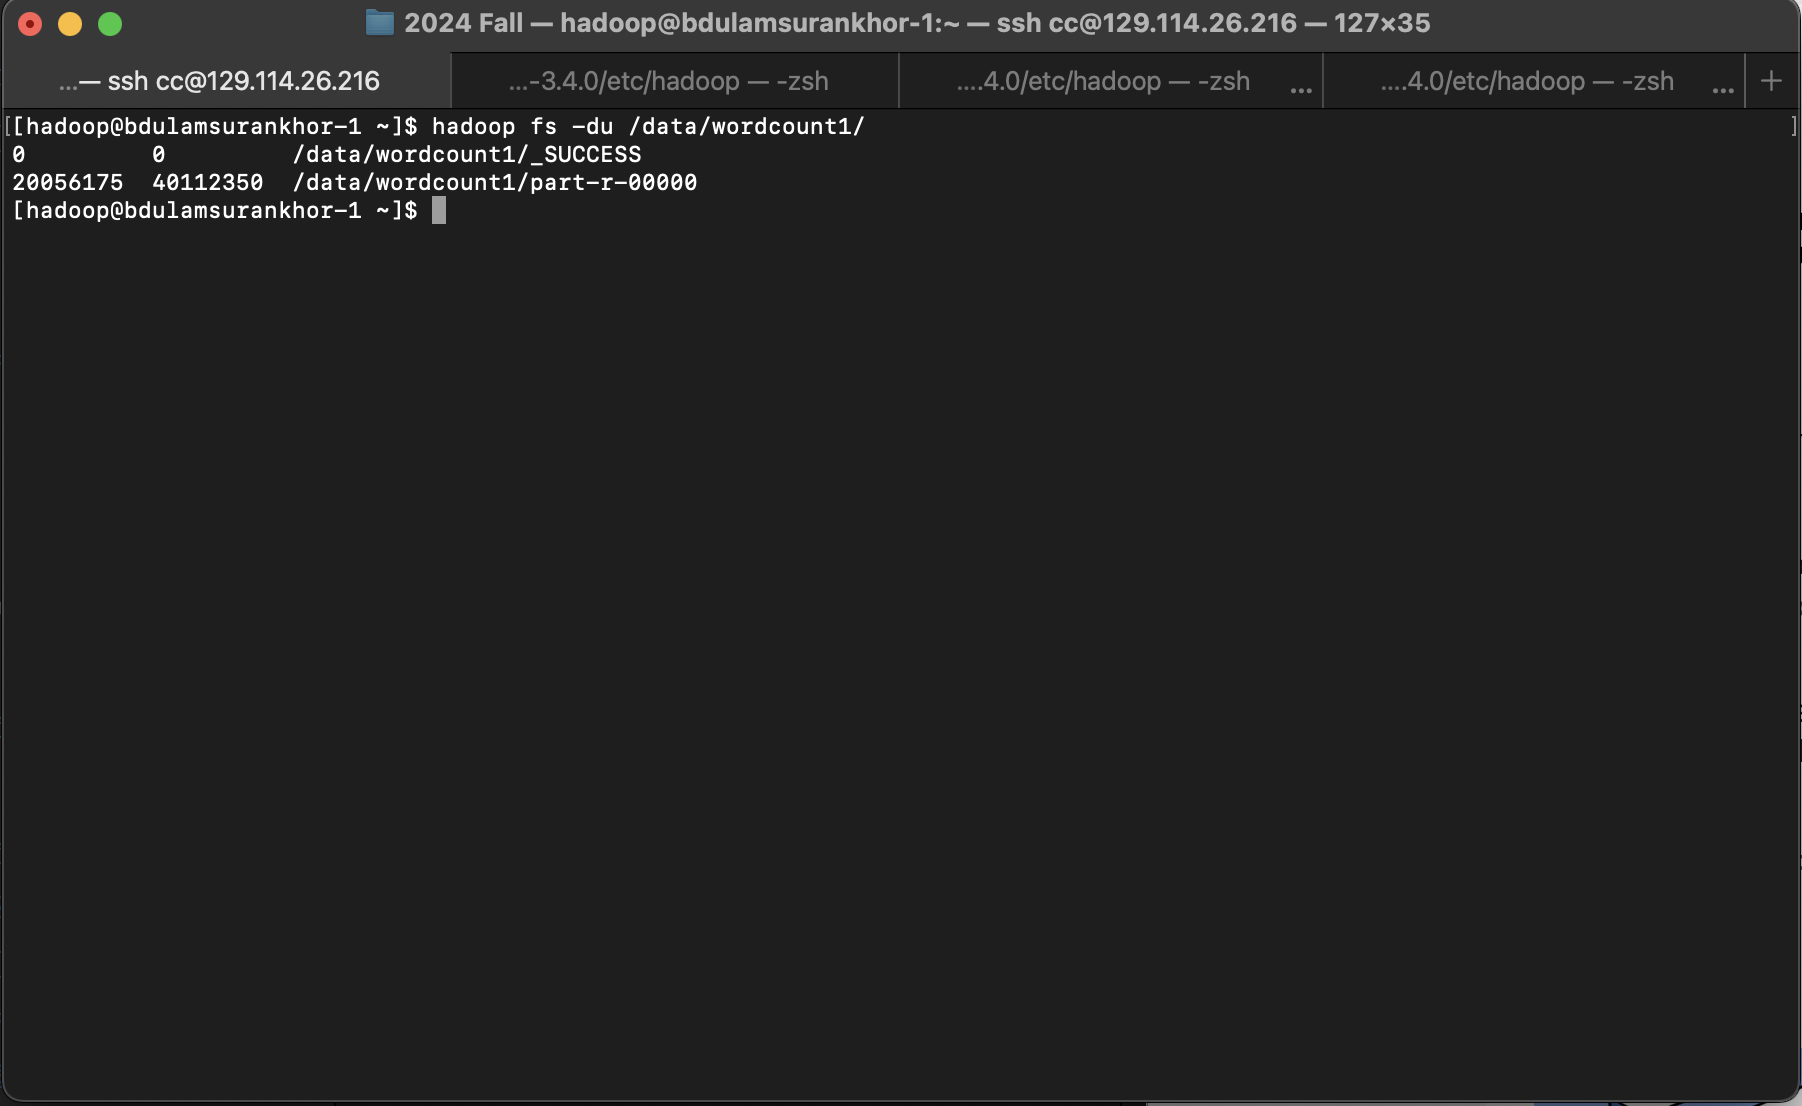
\includegraphics[width=\textwidth]{image5.png}
\end{figure}

hadoop fs -cat /data/wordcount1/part-r-00000 | grep arctic

\begin{figure}[H]
  \centering
  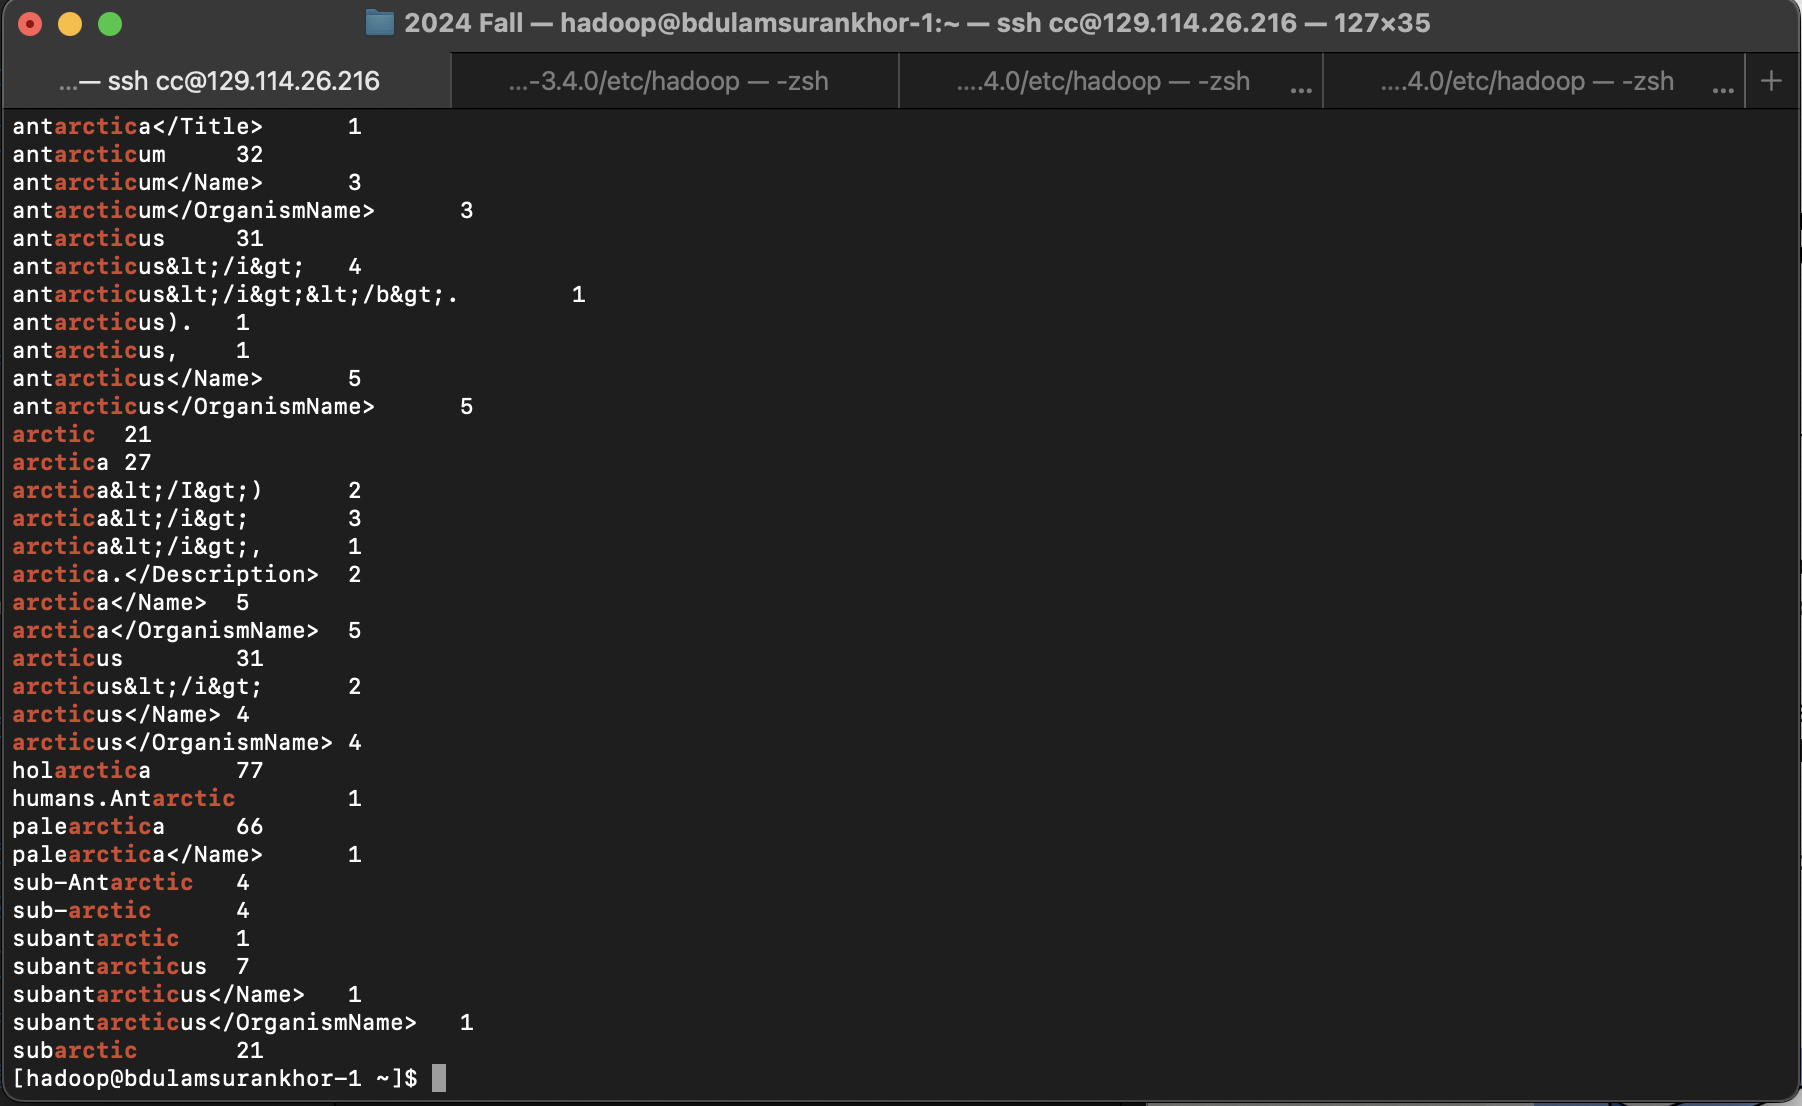
\includegraphics[width=\textwidth]{image6.png}
\end{figure}

6) SELECT COUNT(*) FROM VehicleData;

\begin{figure}[H]
  \centering
  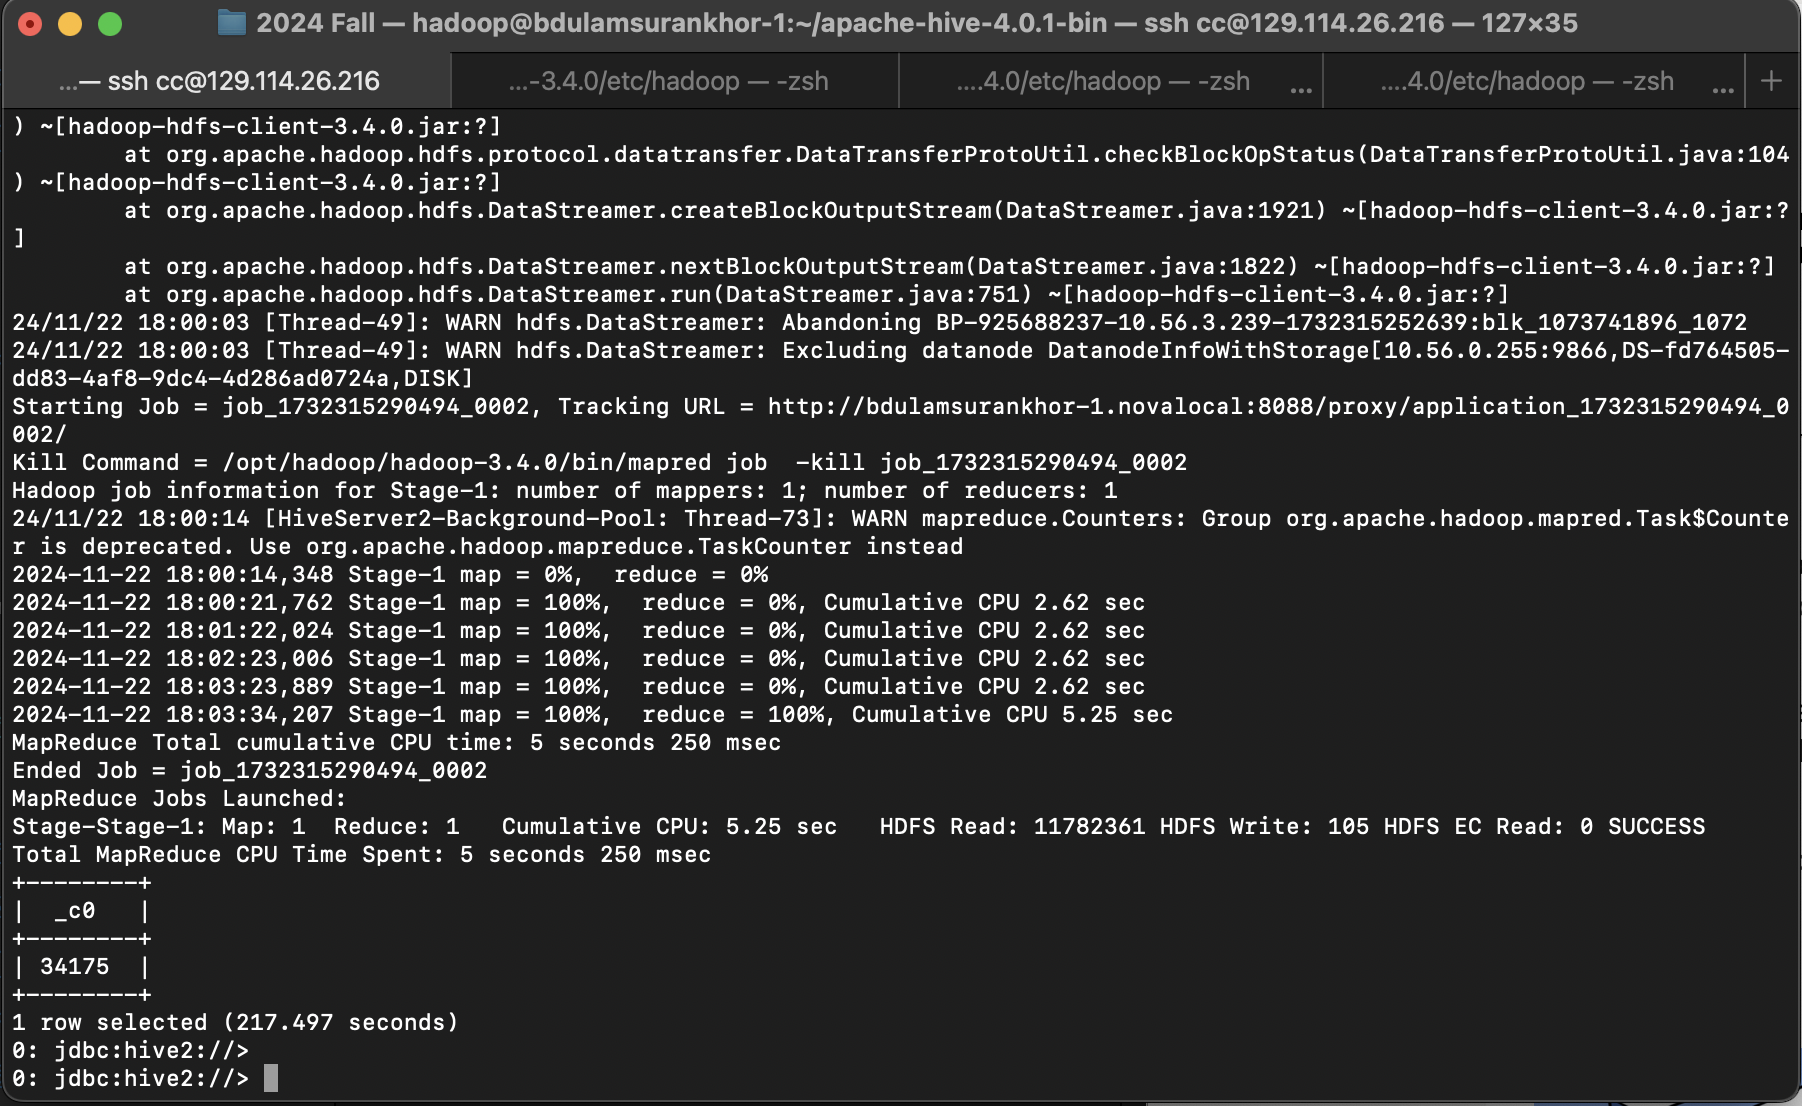
\includegraphics[width=\textwidth]{image8.png}
\end{figure}

SELECT MIN(barrels08), AVG(barrels08), MAX(barrels08) FROM VehicleData;

\begin{figure}[H]
  \centering
  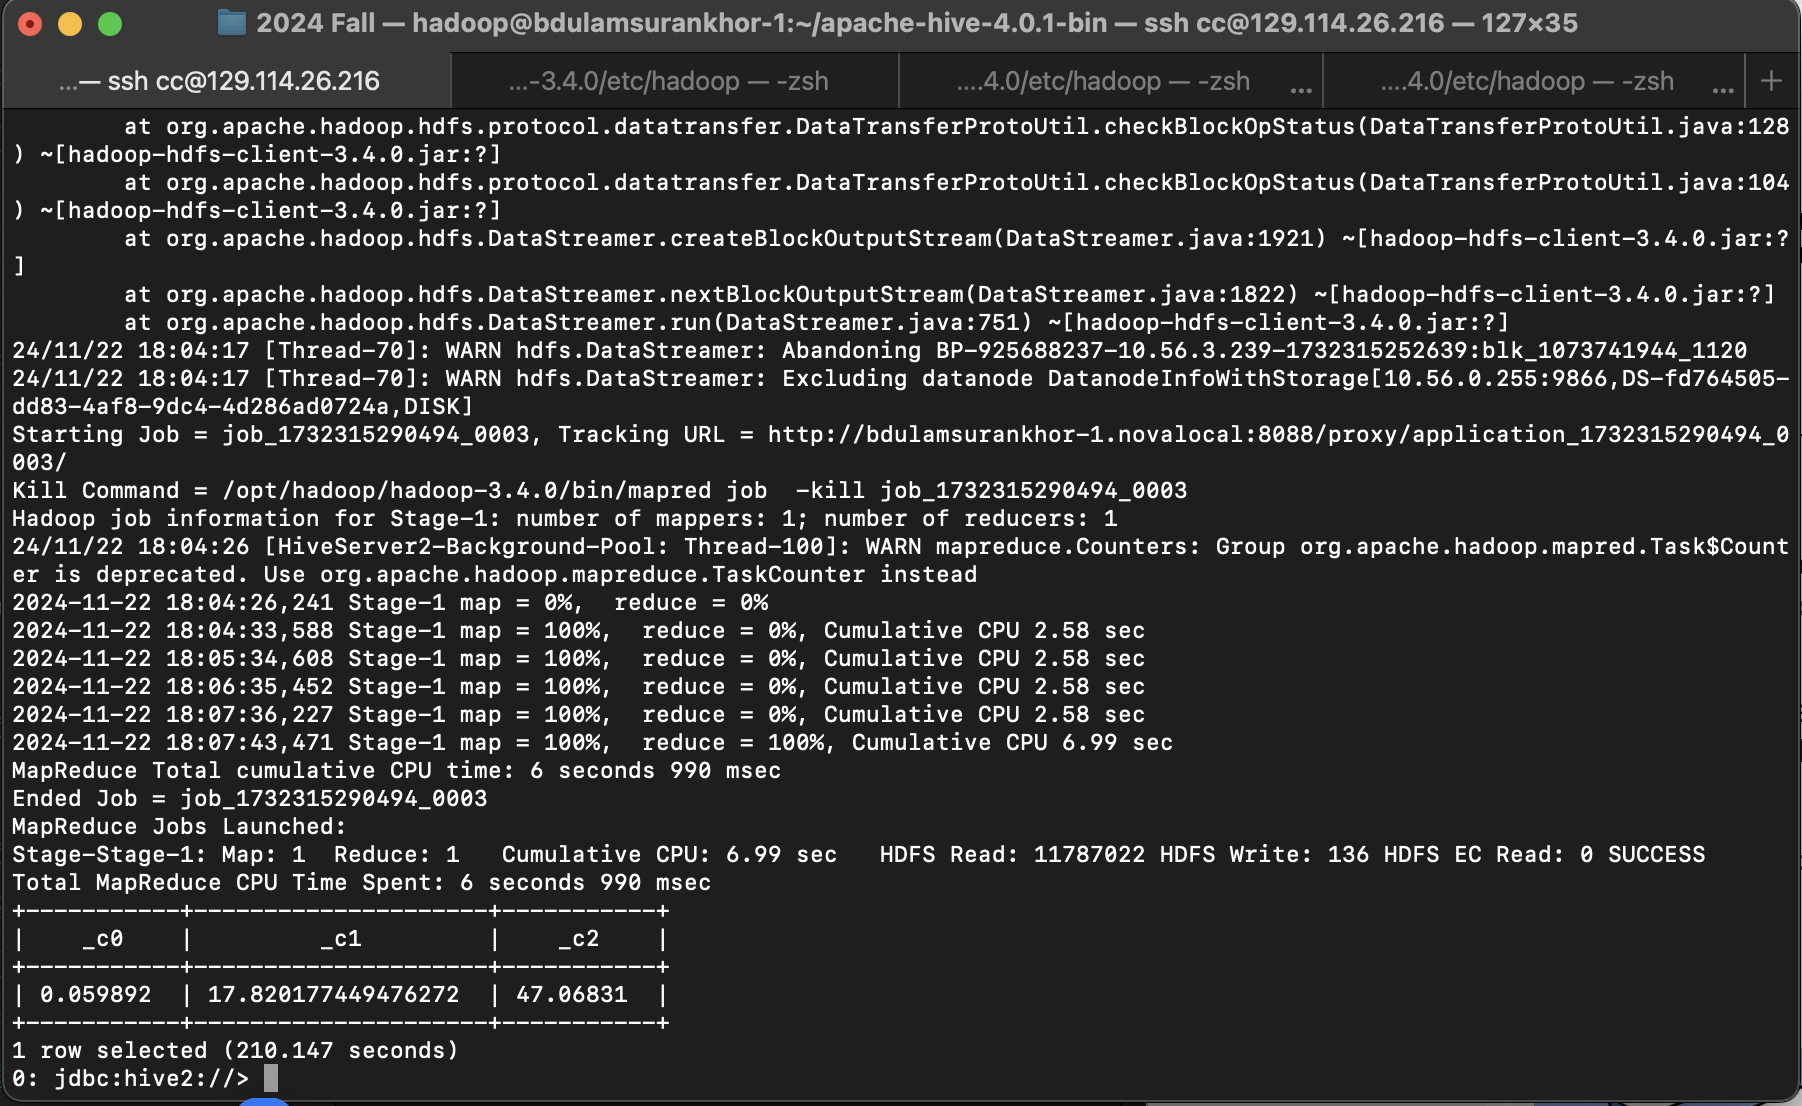
\includegraphics[width=\textwidth]{image9.png}
\end{figure}

SELECT (barrels08/city08) FROM VehicleData;

\begin{figure}[H]
  \centering
  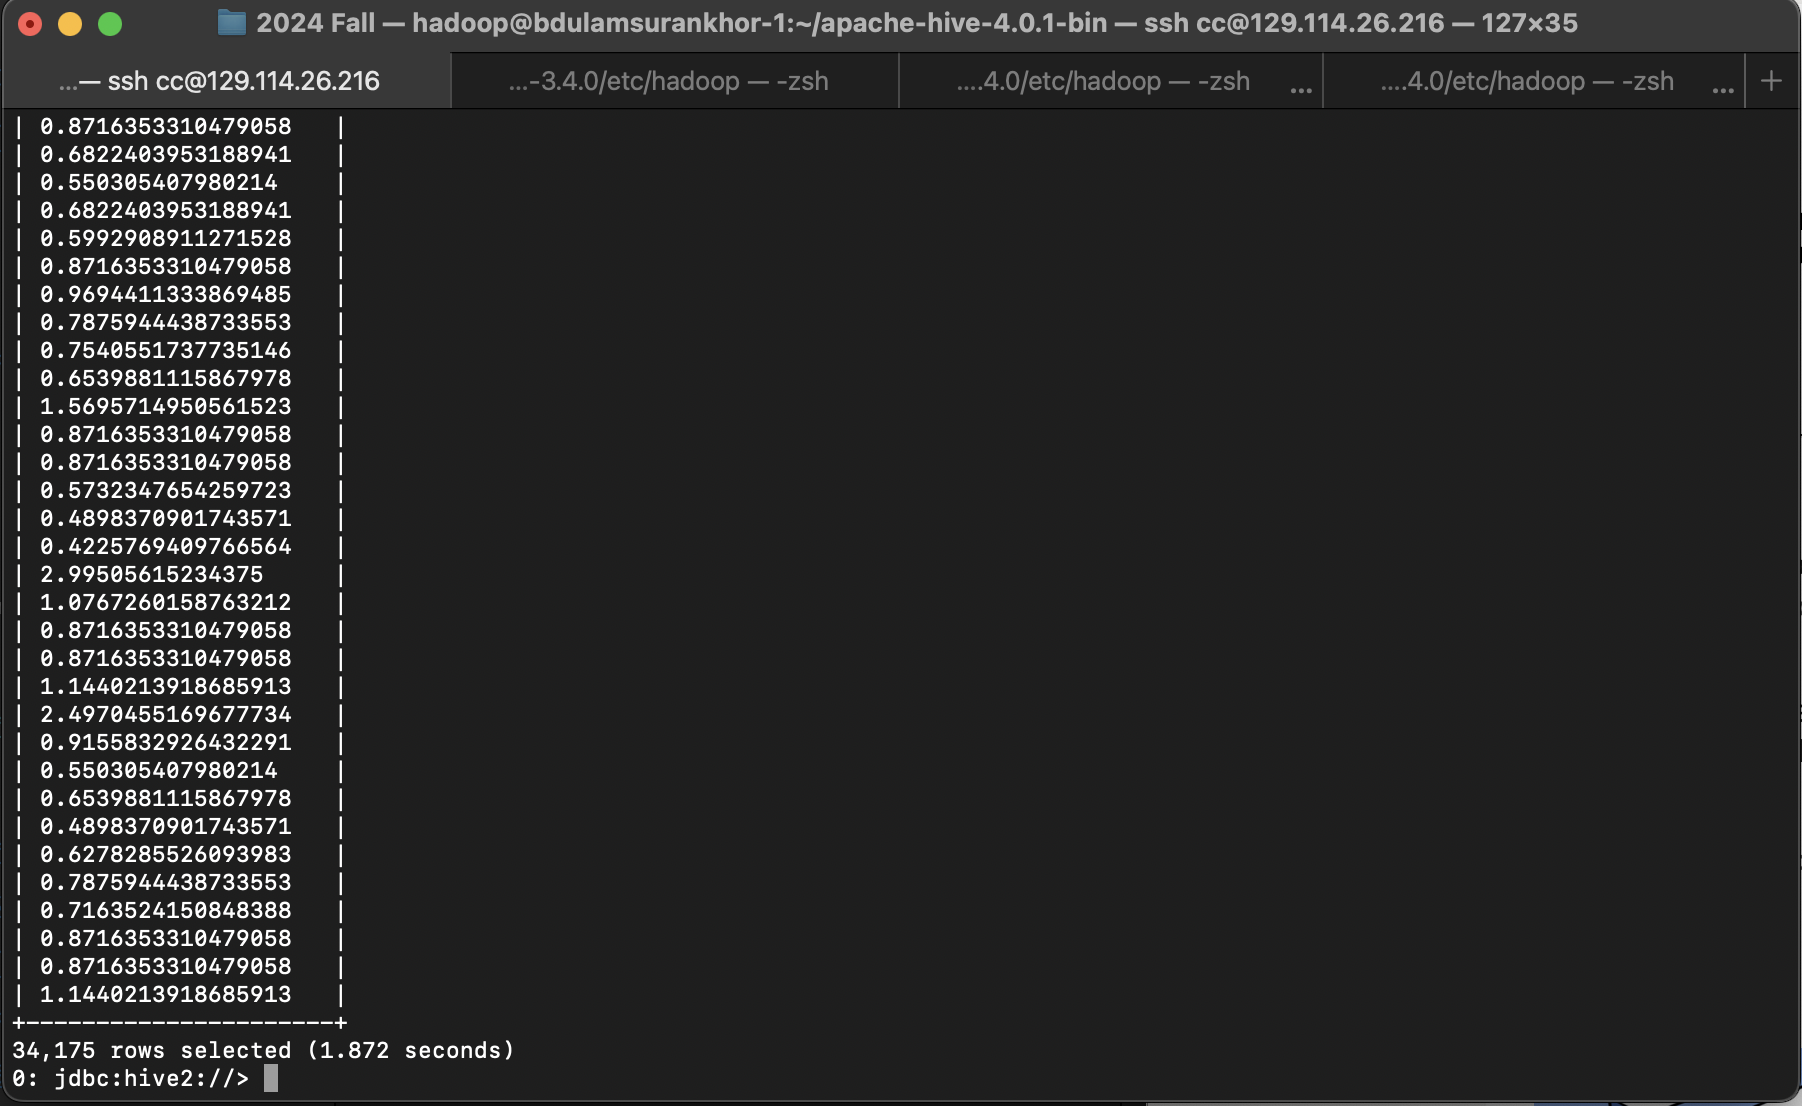
\includegraphics[width=\textwidth]{image10.png}
\end{figure}

INSERT OVERWRITE DIRECTORY 'ThreeColExtract'
SELECT barrels08, city08, charge120
FROM VehicleData;

\begin{figure}[H]
  \centering
  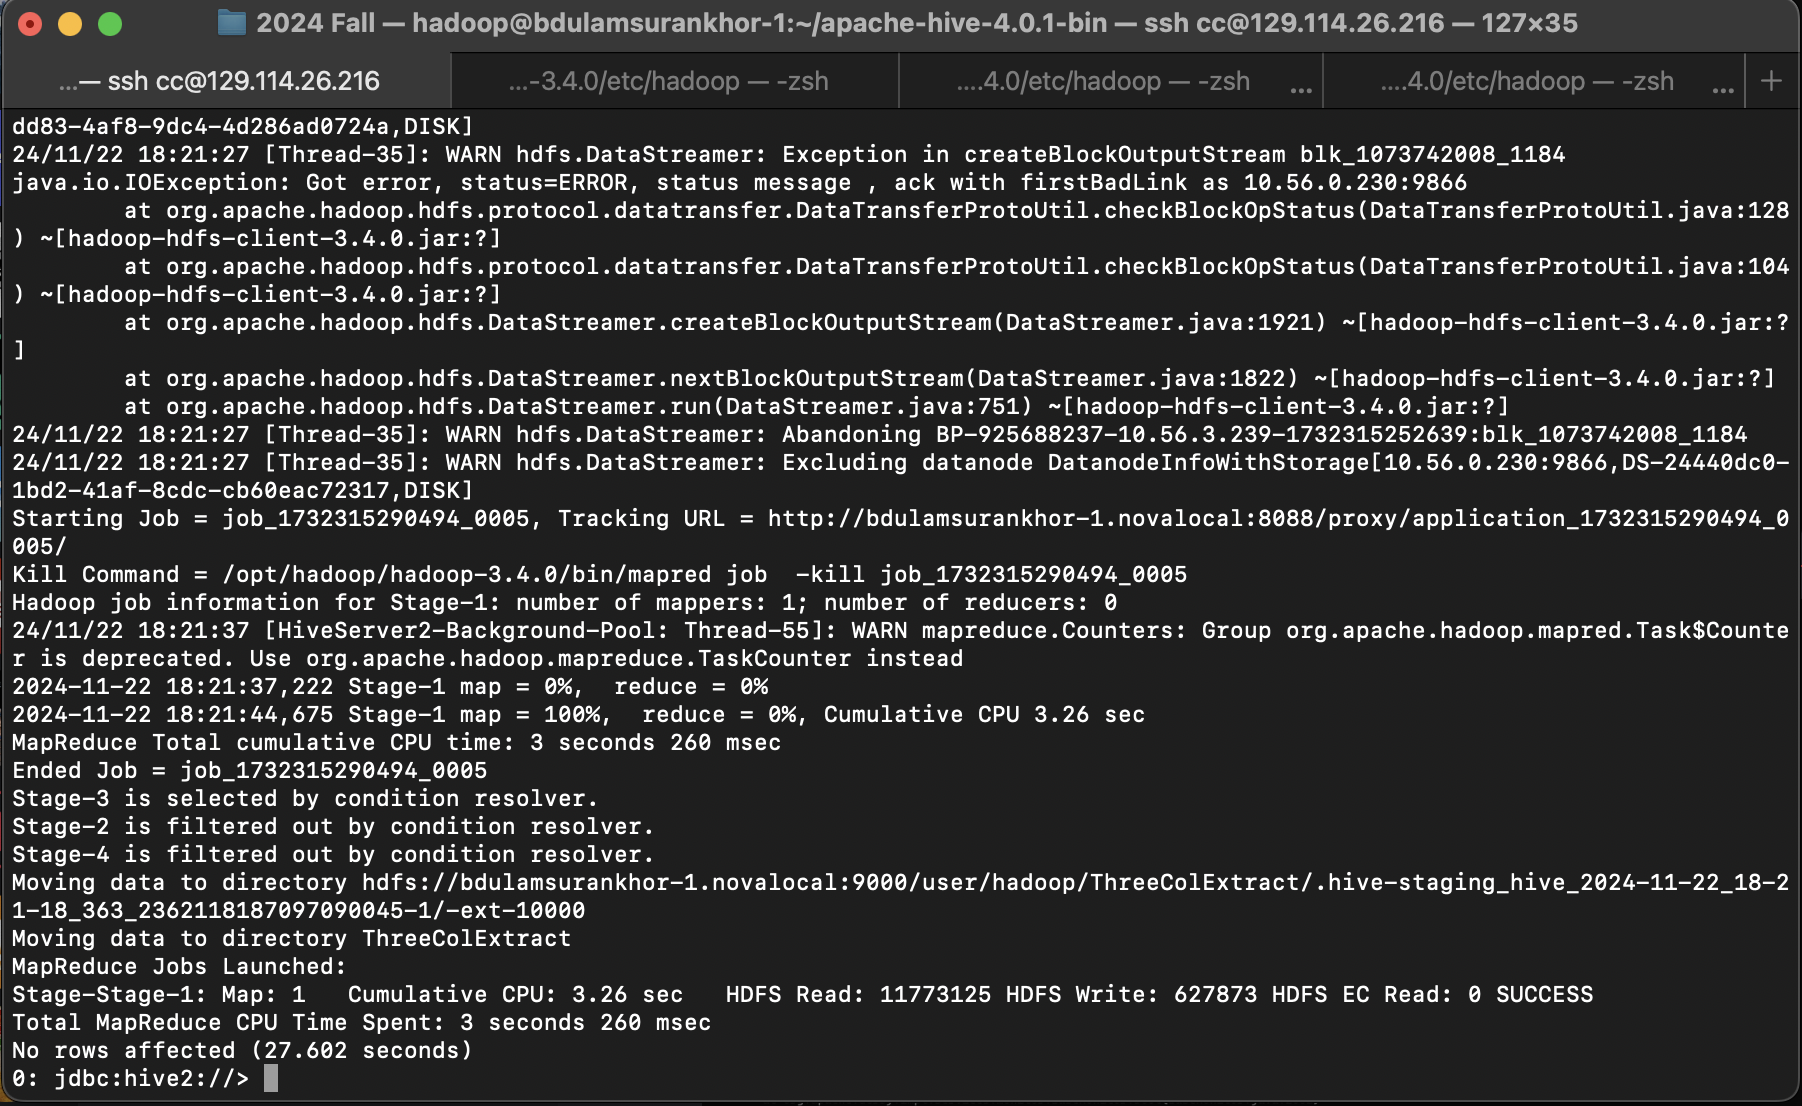
\includegraphics[width=\textwidth]{image11.png}
\end{figure}

hadoop fs -ls ThreeColExtract

\begin{figure}[H]
  \centering
  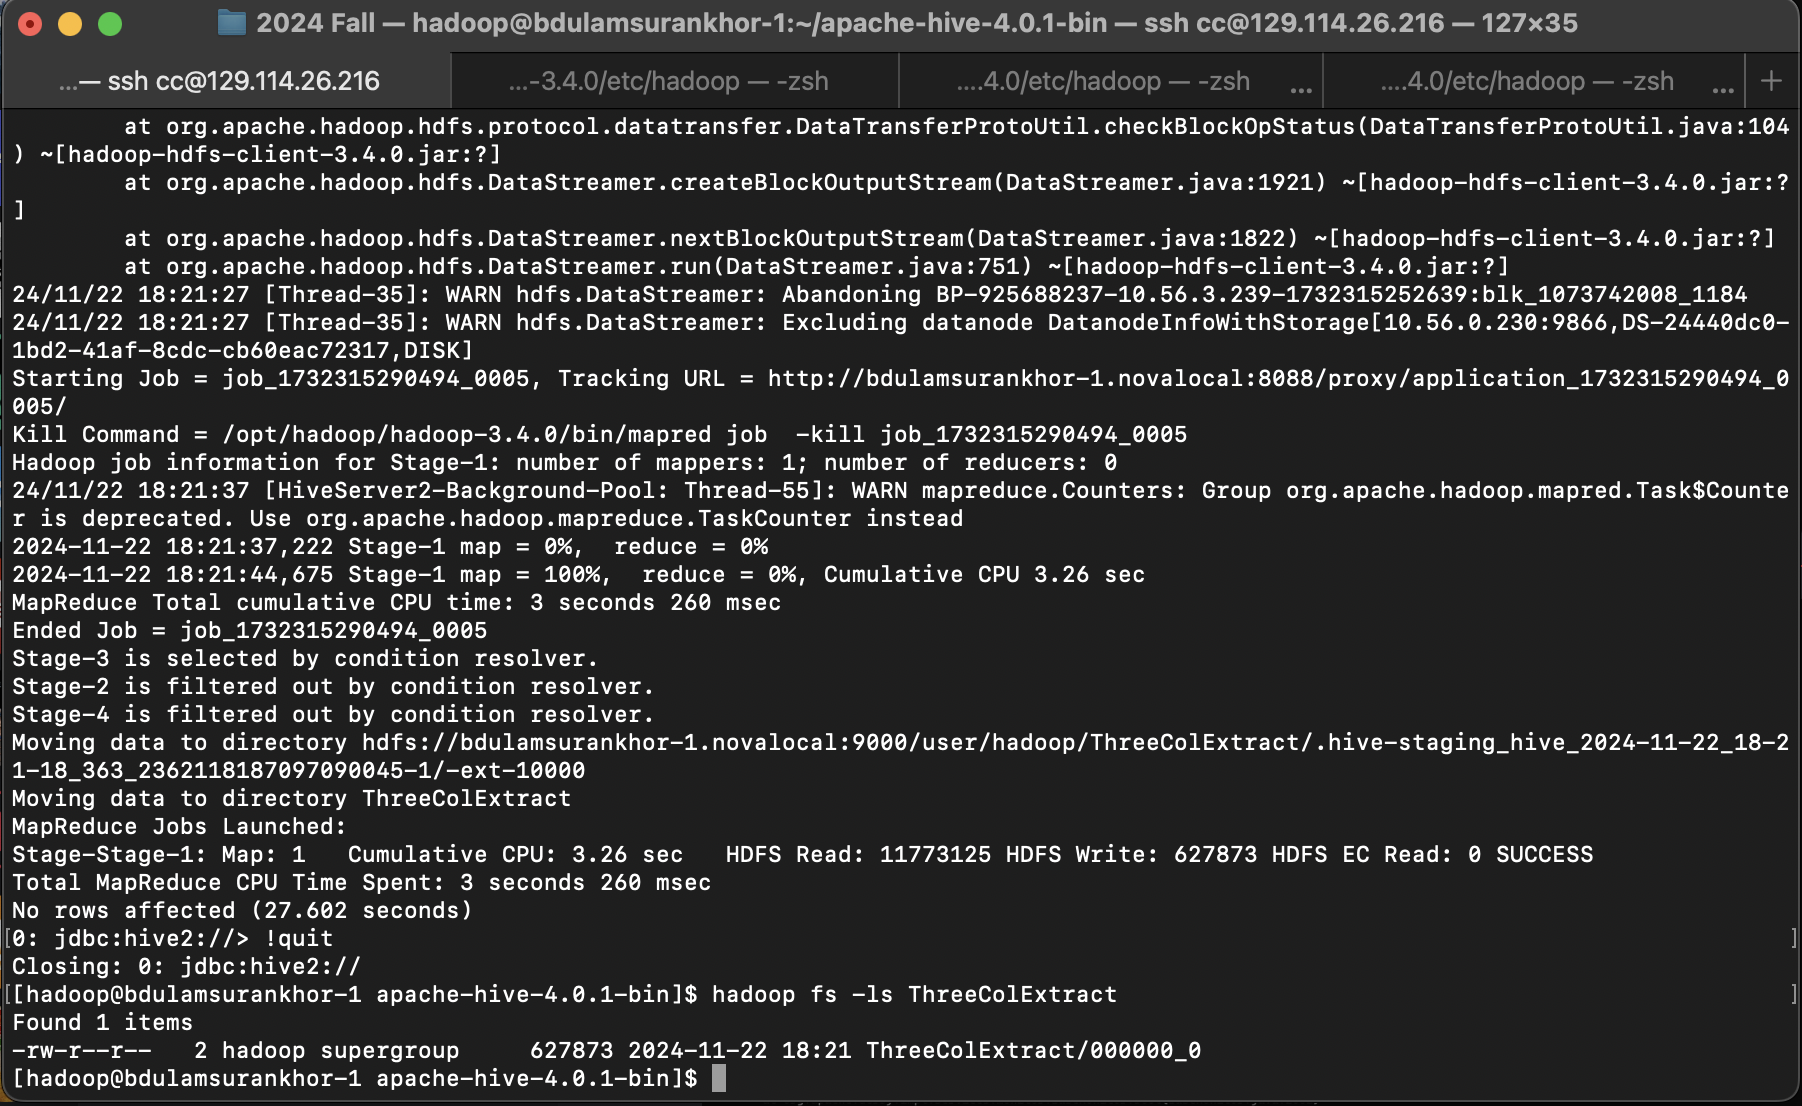
\includegraphics[width=\textwidth]{image12.png}
\end{figure}

Download data:

wget http://cdmgcsarprd01.dpu.depaul.edu/CSC555/SSBM1/lineorder.tbl

Load data:

LOAD DATA LOCAL INPATH '/opt/hadoop/lineorder.tbl' OVERWRITE INTO TABLE lineorder;

\begin{figure}[H]
  \centering
  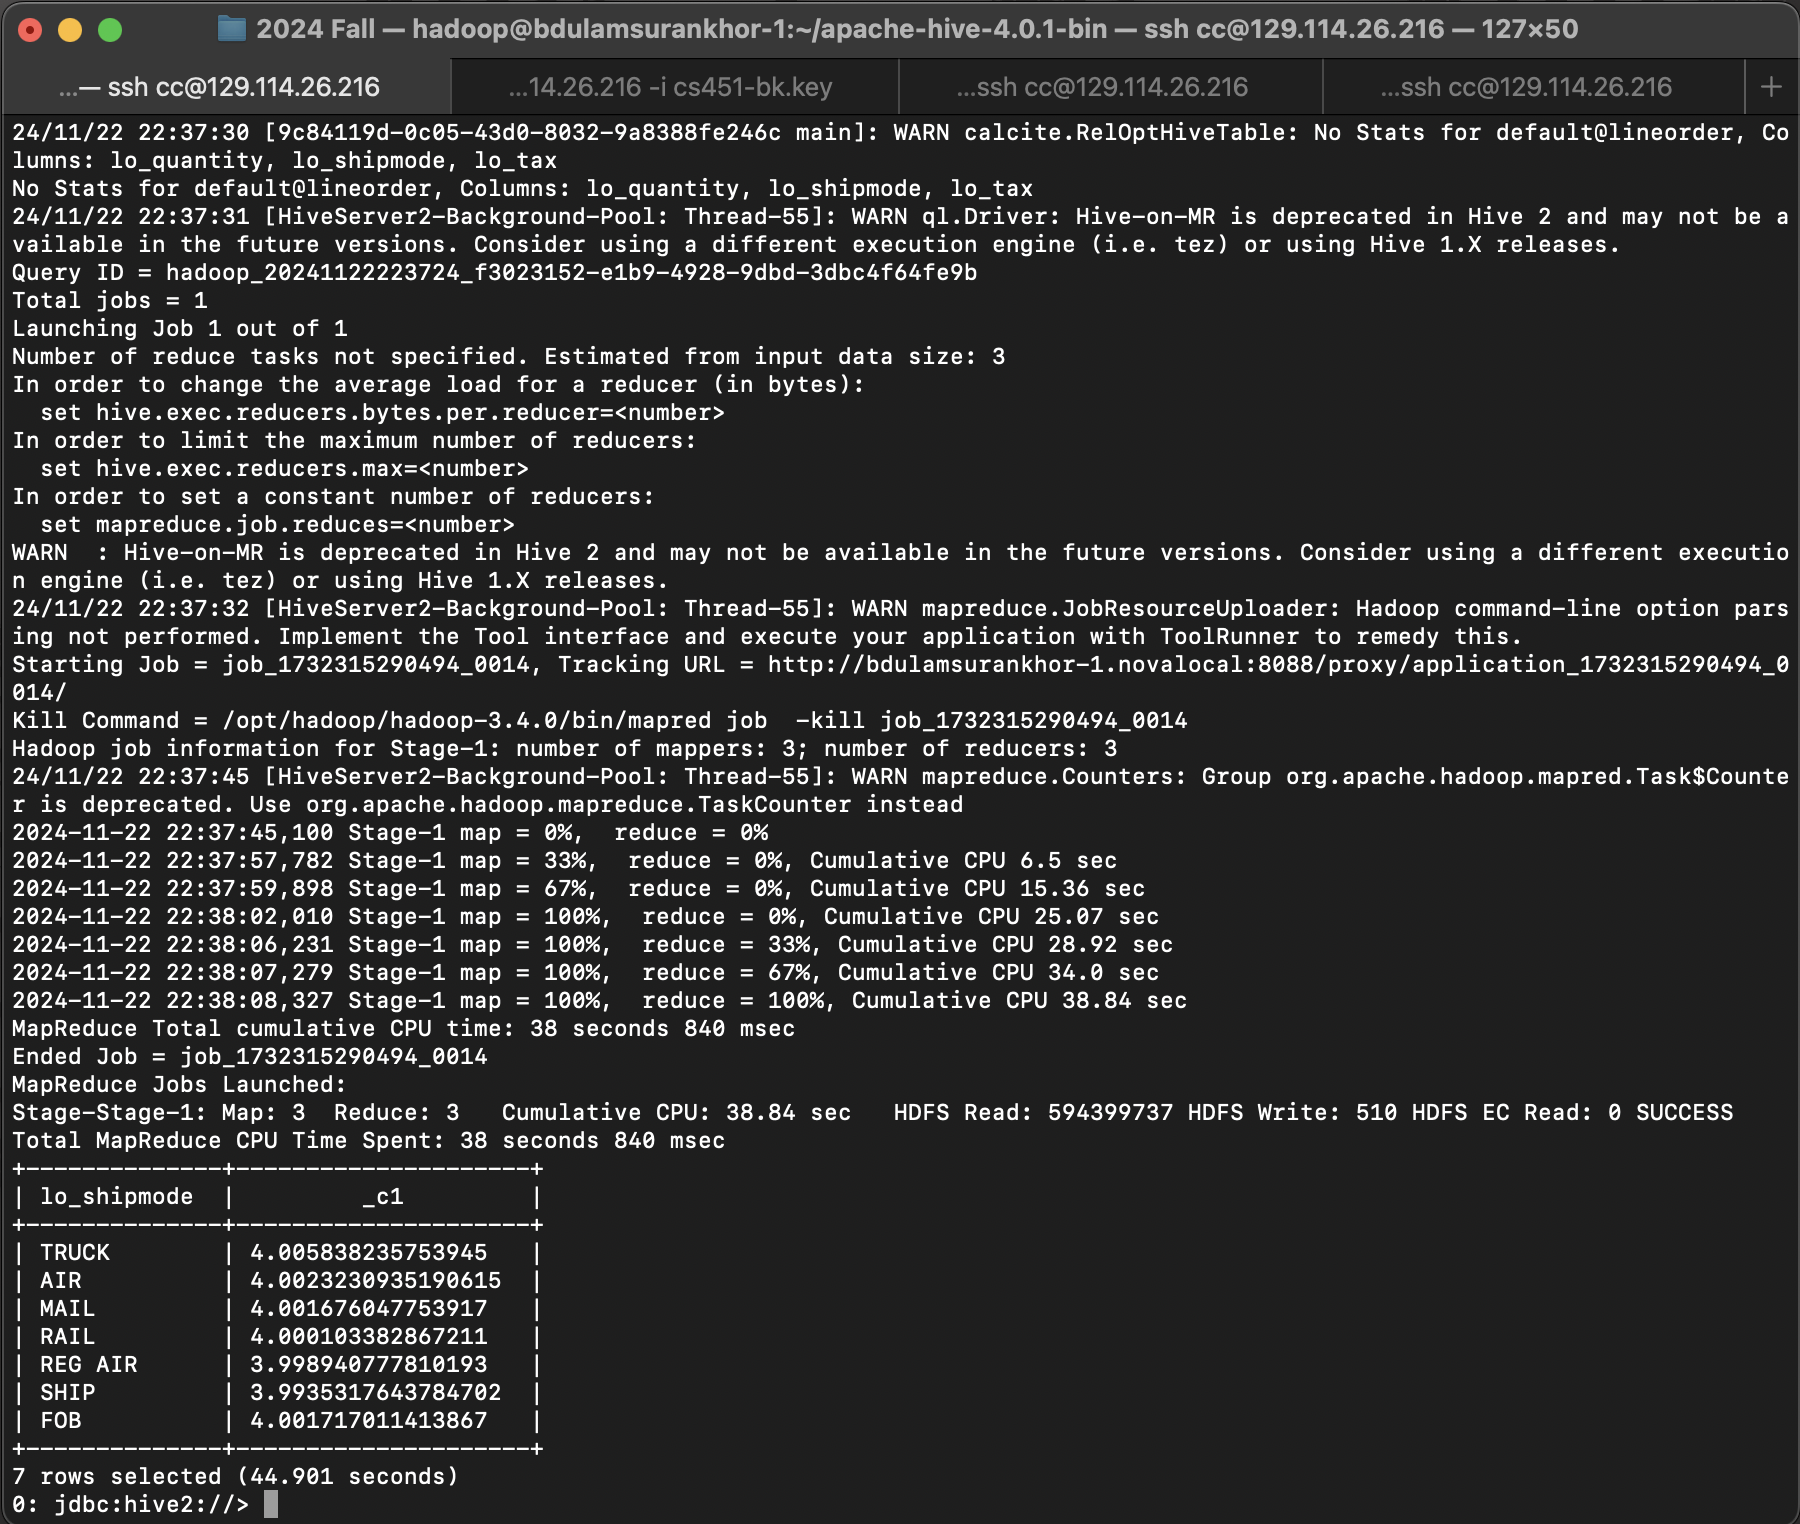
\includegraphics[width=\textwidth]{image13.png}
\end{figure}

7) Use the same vehicles file. Copy the vehicles.csv file to the HDFS if it is not already there.

VehicleData = LOAD '/data/vehicles.csv' USING PigStorage(',') AS (barrels08:FLOAT, barrelsA08:FLOAT, charge120:FLOAT, charge240:FLOAT, city08:FLOAT);

You can see the table description by

DESCRIBE VehicleData;

Verify that your data has loaded by running:

VehicleG = GROUP VehicleData ALL;

Count = FOREACH VehicleG GENERATE COUNT(VehicleData);

DUMP Count;

\begin{figure}[H]
  \centering
  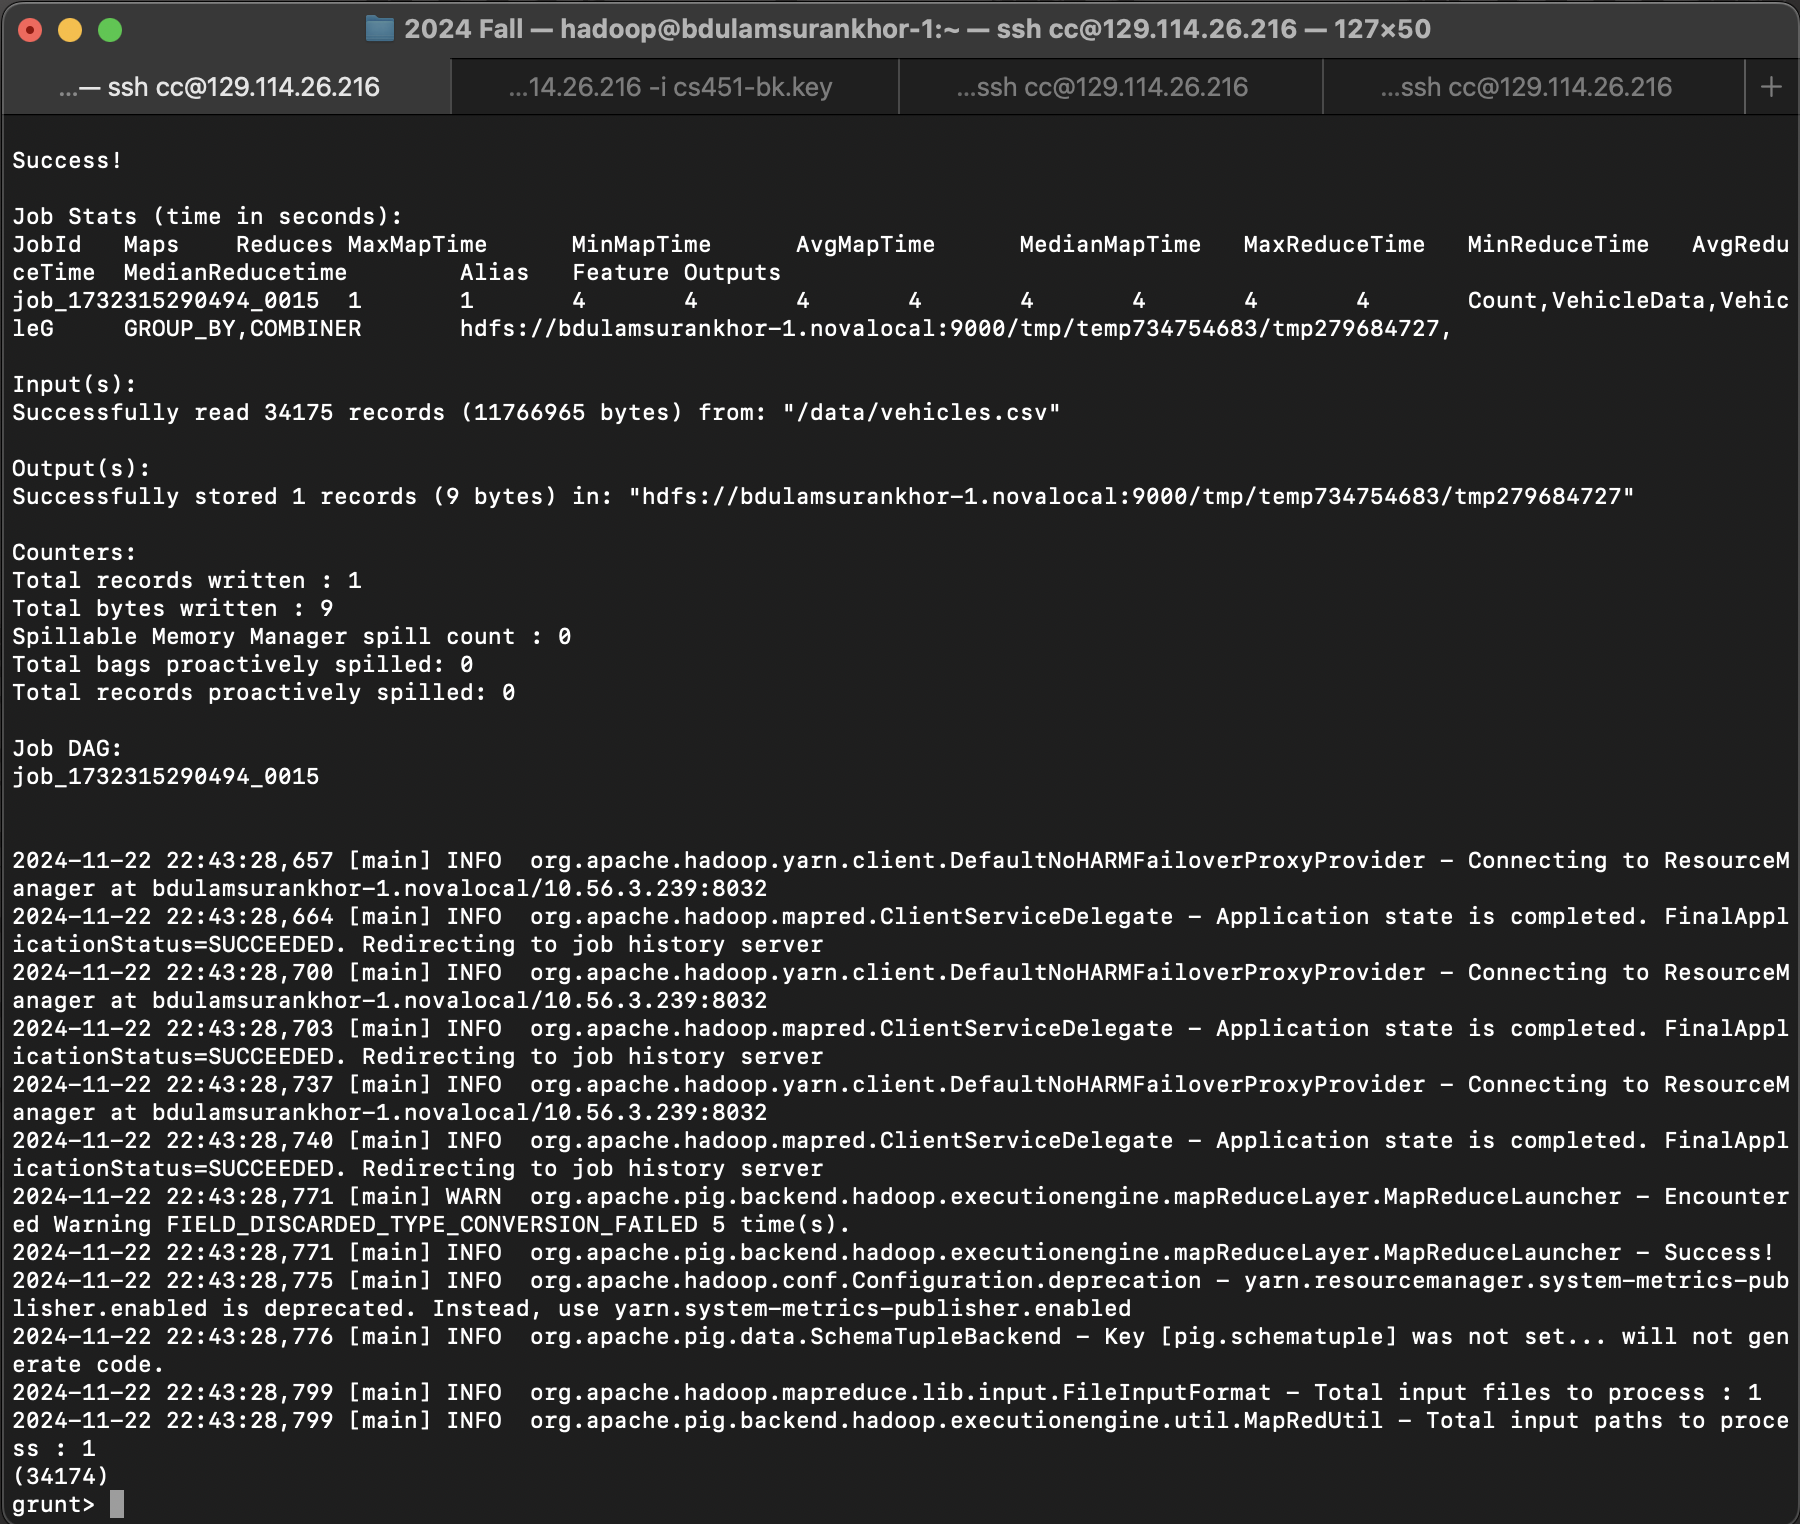
\includegraphics[width=\textwidth]{image14.png}
\end{figure}


\end{document}